\chapter{The Large Hadron Collider (LHC)}

The Large Hadron Collider (LHC) is the world's largest and highest-energy particle accelerator. Straddling the France-Switzerland border at CERN, near Geneva, Switzerland, the LHC is installed in a 26.7 km-long circular tunnel between 45 and 170 m underground. The LHC is a proton-proton ($pp$) collider, designed to accelerate protons to near-light speed (about 3 m/s slower than $c$). The protons are accelerated in two counter-rotating beams, each housed inside vacuum tubes and bent into a ring by 8.3 T superconducting magnets. At detector locations, the beams are crossed so that collisions may occur. An overview of the experiments on the LHC ring can be seen in Figure~\ref{fig:LHCRing}. 

\begin{figure}\centering
  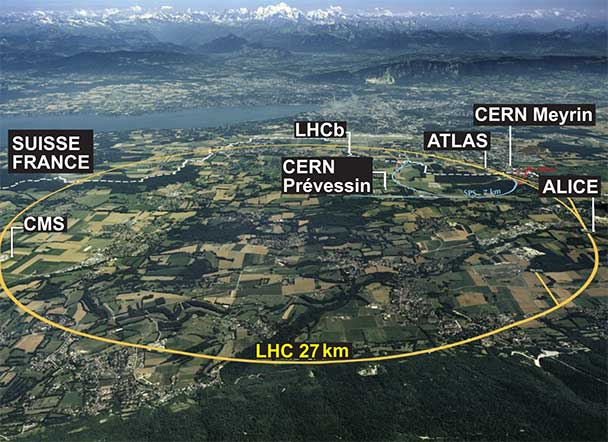
\includegraphics[width=1.0\textwidth]{figures/LHCRing.jpg}
  \caption{\label{fig:LHCRing} The Large Hadron Collider located underneath the Franco-Swiss border at CERN near Geneva, Switzerland. The CMS Experiment is located on the French side in Cessy, France}
\end{figure}

The protons are divided into ``bunches" by radio-frequency (RF) cavities, with about $10^{11}$ protons per bunch. Each beam contains 2808 bunches. The design center of mass collision energy is $\sqrt{s} = 14$ TeV, which corresponds to 7 TeV per colliding proton bunch. The LHC is designed for bunch spacings of about 25 ns, corresponds to a design collision rate of about 40 MHz. The design instantaneous luminosity (number of protons in a collision area per unit time) of the LHC is $\mathcal{L} = 10^{34}$ cm$^{-2}$ s$^{-1}$. Integrated over time, the instantaneous luminosity gives the \textit{integrated luminosity}:

\begin{equation}
L = \int\mathcal{L}(t)dt
\end{equation}

Over the 2012 run, during which time the LHC was running at a $pp$ collision energy of $\sqrt{s} = 8$ TeV and a bunch spacing of 50 ns, the LHC delivered 23.3 fb$^{-1}$ of integrated luminosity, of which CMS recorded 21.8 fb$^{-1}$. During the 2015 run, during which time the LHC was running at a $pp$ collision energy of $\sqrt{s} = 13$ TeV and a bunch spacing of 25 ns, the LHC delivered 4.22 fb$^{-1}$ of integrated luminosity, of which CMS recorded 3.81 fb$^{-1}$. As of this writing, the LHC is wrapping up its 2016 run, also with a $pp$ collision energy of $\sqrt{s} = 13$ TeV and a bunch spacing of 25 ns, and so far 34.1 fb$^{-1}$ of instantaneous luminosity have been delivered and 31.4 fb$^{-1}$ have been recorded by CMS. A plot of the luminosity delivered so far during 2016 is shown in Figure \ref{fig:LumiPlot}.

\begin{figure}\centering
  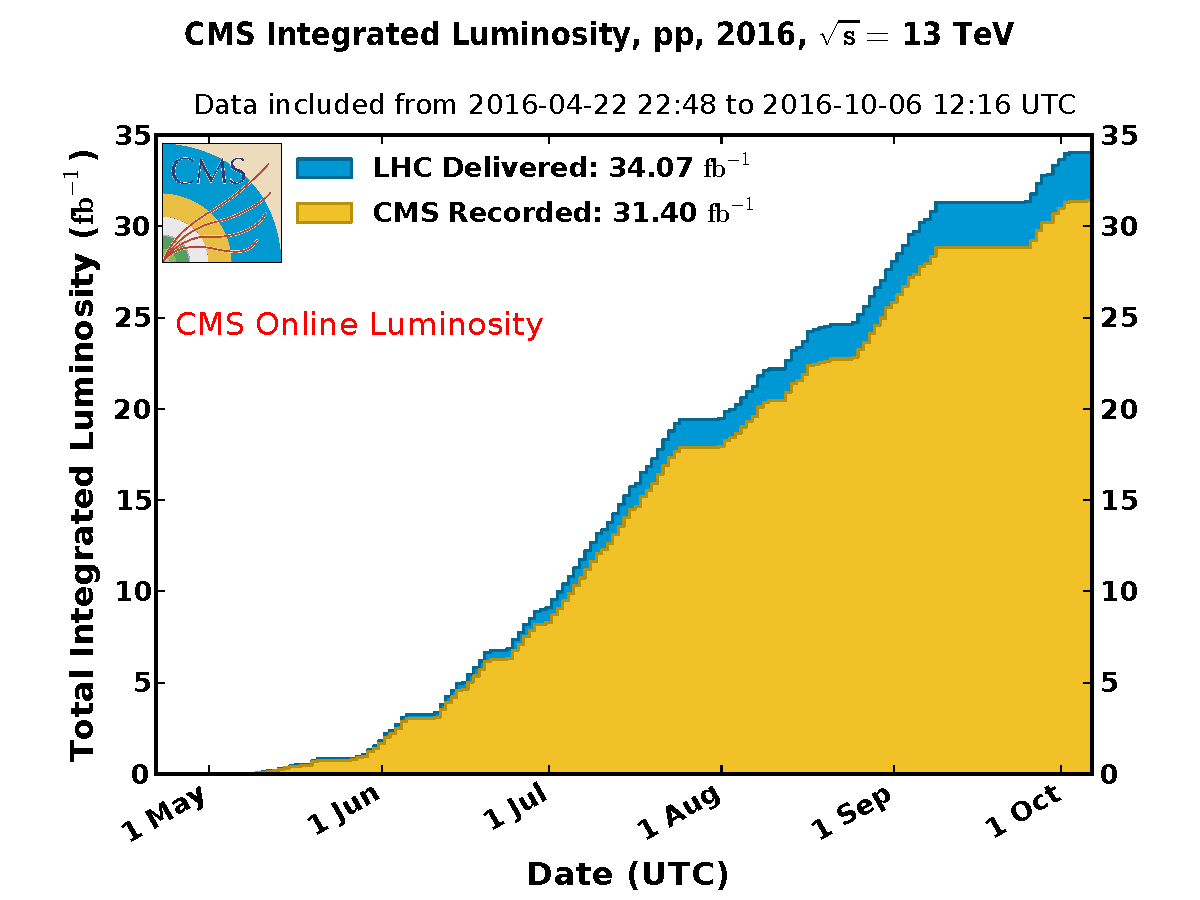
\includegraphics[width=1.0\textwidth]{figures/LumiPlot.pdf}
  \caption{\label{fig:LumiPlot} Total integrated luminosity delivered by the LHC (blue), and total integrated luminosity recorded by CMS (yellow) during the 2016 run.}
\end{figure}


\chapter{The Compact Muon Solenoid}

The Compact Muon Solenoid (CMS) Experiment is a multipurpose particle detector located on the LHC ring underneath the France-Switzerland border at CERN near Geneva, Switzerland. The CMS experiment is located 100 meters underground in Cessy, France and is 28.7 meters long, 15.0 meters in diameter, and weighs approximately 14,000 tonnes. It is arranged in a cylindrical, multi-layered structure consisting of a ``barrel" and two endcaps, with the LHC beam passing through the central axis of the cylinder. The central feature of the CMS apparatus is a superconducting solenoid of 6 m internal diameter, providing a magnetic field of 3.8 T. Within the solenoid volume are a silicon pixel and strip tracker, a lead tungstate crystal electromagnetic calorimeter (ECAL), and a brass and scintillator hadron calorimeter (HCAL), each composed of a barrel and two endcap sections. Forward calorimeters extend the pseudorapidity coverage provided by the barrel and endcap detectors. Muons are measured in gas-ionization detectors embedded in the steel flux-return yoke outside the solenoid. A photograph of CMS can be seen in Figure~\ref{fig:CMSphoto}, and a diagram highlighting the layout of CMS can be seen in Figure~\ref{fig:CMSdiagram}.
\begin{figure}\centering
  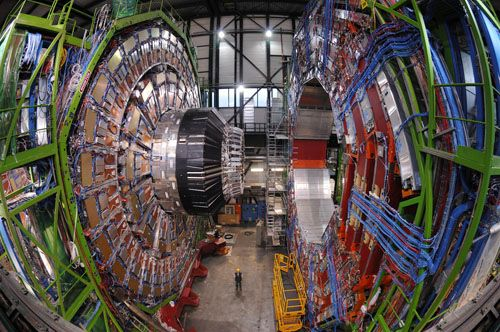
\includegraphics[width=1.0\textwidth]{figures/CMSphoto.jpg}
  \caption{\label{fig:CMSphoto} The CMS Experiment (open for maintenance)}
\end{figure}
The experiment uses a right-handed coordinate system: the origin is set at the $pp$ collision point, with the $x$-axis pointing towards the center of the LHC ring, the $y$-axis pointing up, and the $z$-axis pointing along the beam line in the counter-clockwise direction. CMS also uses a pseudo-polar coordinate system, with $\theta$ defined as the polar angle from the beam axis, and $\eta$ as the ``pseudorapidity", itself defined as 
\begin{equation}
 \eta = -\ln\left[\tan\left(\theta/2\right)\right]
 \end{equation}
\begin{figure}\centering
  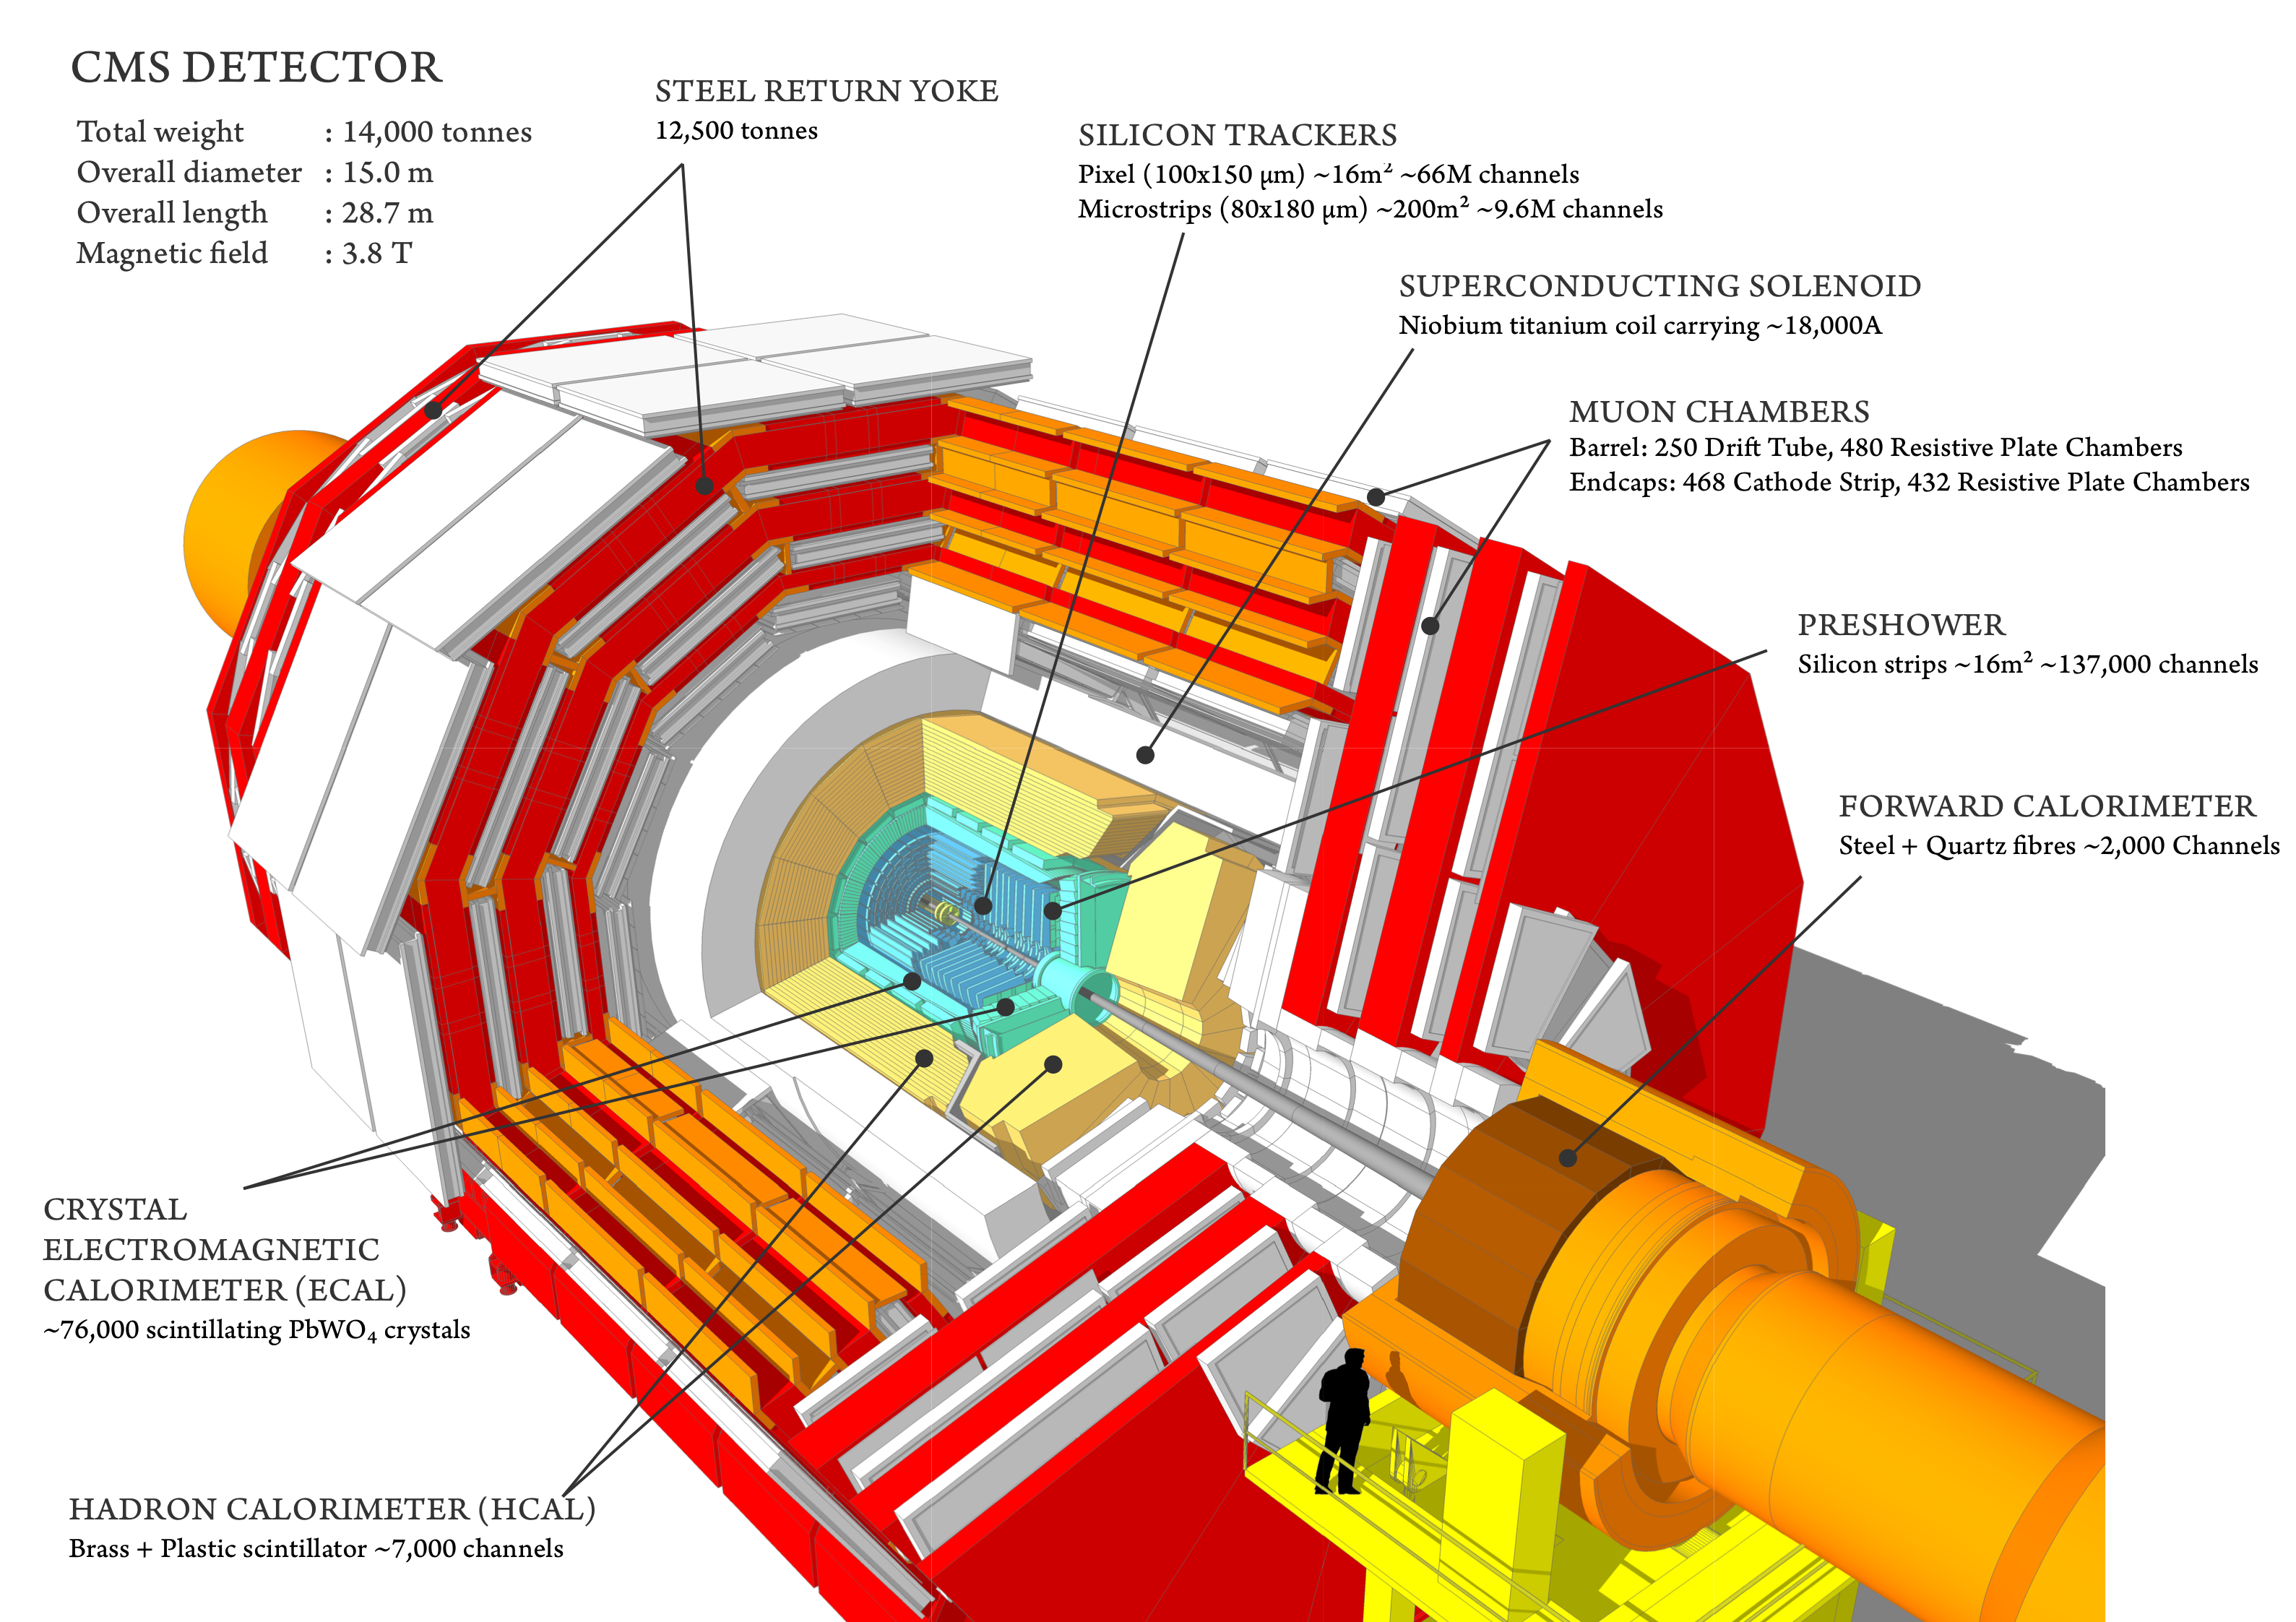
\includegraphics[width=1.0\textwidth]{figures/CMSdiagram.png}
  \caption{\label{fig:CMSdiagram} Schematic of the CMS Experiment showing the silicon trackers, electromagnetic calorimeter (ECAL), hadronic calorimeter (HCAL), superconducting solenoid, steel magnetic flux return yoke, and muon system.}
\end{figure}

\section{The Silicon Tracker}

The silicon tracker is the innermost detector element in CMS, and is designed to provide the highest resolution measurement of charged particle trajectories (such trajectories are referred to as ``tracks"). The tracker is composed of approximately 200 m$^{2}$ of silicon, and includes arrays of silicon pixels in the inner layers and arrays of silicon strips in the outer layers. The total number of channels is 66 million pixels and 9.6 million strips.\cite{TDR} The tracker is divided into a barrel segment and two forward endcaps. The pixel barrel consists of three co-axial layers at radii between 4.4 cm and 10.2 cm, and the strip barrel consists of a further ten co-axial layers extending out to a radius of 110 cm. The pixel endcaps contain two small disks each, while the strip endcaps each consist of three small disks and nine large disks. A schematic of the tracker layout can be seen in Figure~\ref{fig:TrackerLayout}. Particle trajectories are reconstructed by fitting hits in the individual silicon pixels/strips to an interpolated track.

\begin{figure}\centering
  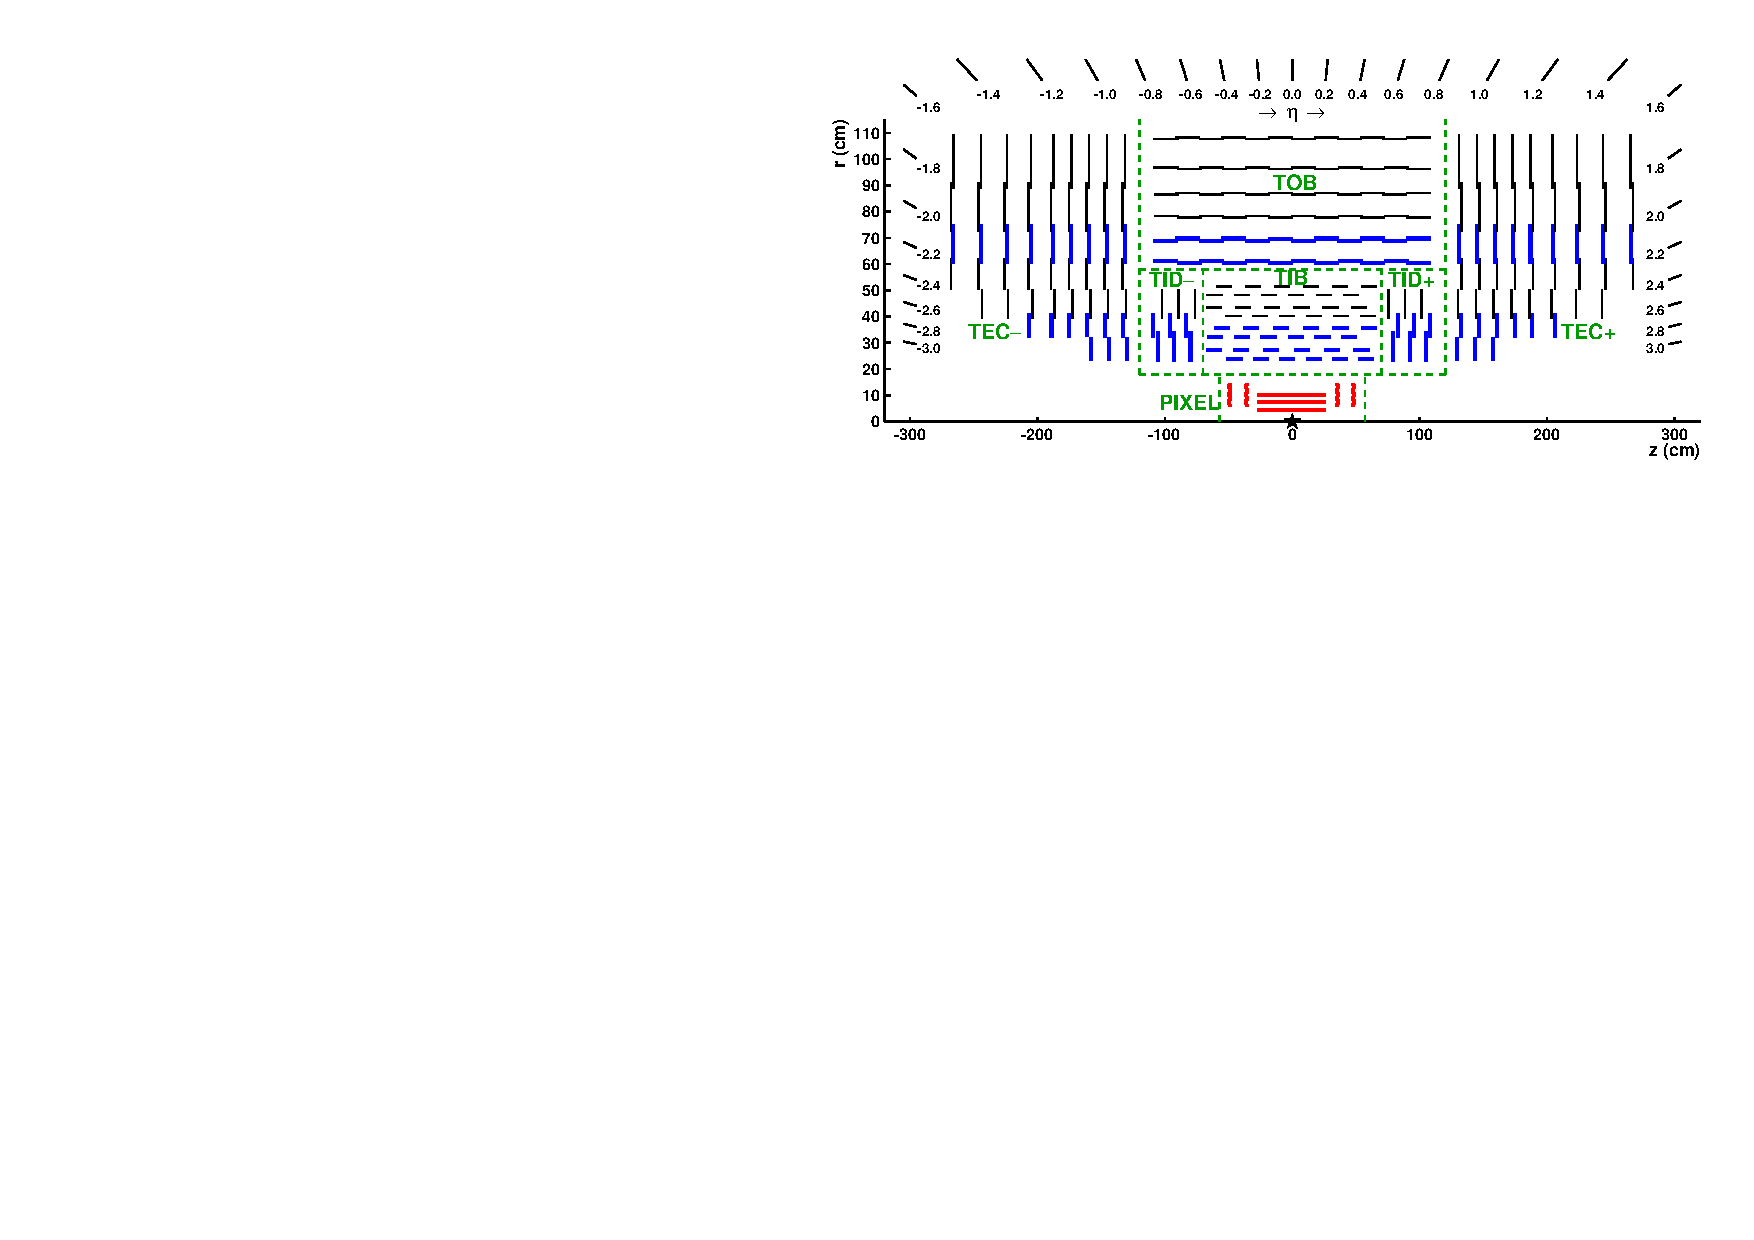
\includegraphics[width=1.0\textwidth]{figures/TrackerLayoutNew.pdf}
  \caption{\label{fig:TrackerLayout} Overview of the silicon tracker layout, including the pixel layers and disks (red), the TIB and TOB layers, and the TID and TEC disks.}
\end{figure}


\subsection{The Pixel Detector}

The pixel detector, shown in Figure ~\ref{fig:PixelLayout}, consists of three barrel layers and two endcap disks on each side. The barrel has a length of 53 cm, and the endcap disks range from 6 cm to 15 cm in radius. The pixel modules are arranged in a ladder-like configuration in the barrel, with 768 total modules comprising the barrel. The endcap disks are arranged in a turbine-like fashion, with 24 ``blades" per disk, and 7 pixel modules per blade for a total of 672 pixel modules in the endcaps.
Each pixel module consists of either 8 or 16 readout chips (ROCs), which are bump bonded to the module. In total, the pixel detector includes about 16,000 ROCs.\cite{Pixel}

\begin{figure}\centering
  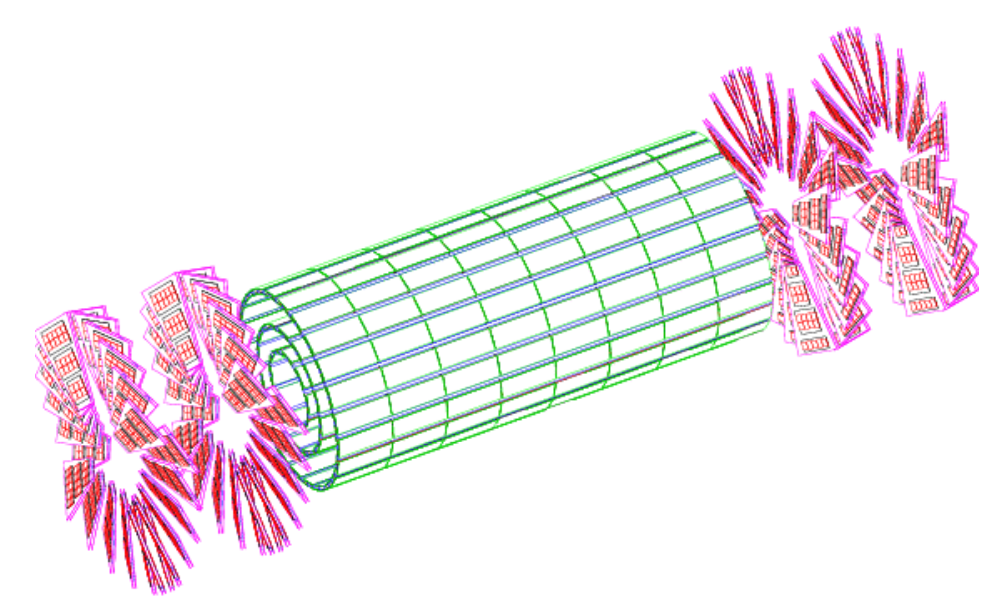
\includegraphics[width=1.0\textwidth]{figures/PixelLayout.png}
  \caption{\label{fig:PixelLayout} Diagram indicating the layout of the barrel pixel (BPIX) sensors (in green) and endcap pixel (FPIX) sensors (in pink)}
\end{figure}

\subsubsection{Pixel Detector Performance}

Common measurements of the detector performance are hit efficiency (Figure~\ref{fig:PixelEfficiency}) and hit resolution (Figure~\ref{fig:PixelResolution}). Hit efficiency is defined as the probability of finding any hit clusters within a 500 $\mu$m$^2$ area around an expected hit, where an expected hit is provided by a ``good quality track" with an associated primary vertex (PV), small impact parameter with respect to that vertex, and $p_{T} > 1.0$ GeV. ``Primary vertex" refers to the reconstructed origin of the tracks corresponding to the $pp$ collision, and will be discussed in further detail in Section \ref{sec:TrackReco}. ``Impact parameter" refers to the distance between the PV and the point of closest approach between the PV and the track. The hit resolution is measured by comparing the hit position on a given layer with an interpolated track and taking the residual difference.\cite{PixelPerformance}

\begin{figure}\centering
  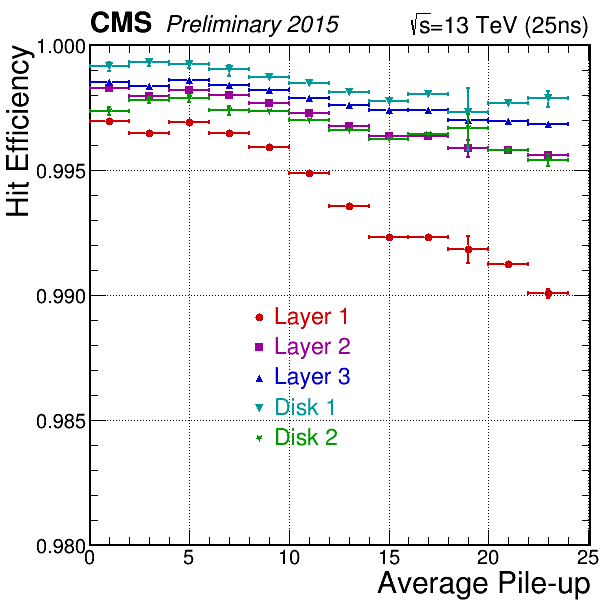
\includegraphics[width=0.5\textwidth]{figures/PixelEfficiency.png}
  \caption{\label{fig:PixelEfficiency} Hit efficiency vs. the average number of inelastic proton-proton collisions for pixel barrel layers and forward disks.}
\end{figure}

\begin{figure}\centering
  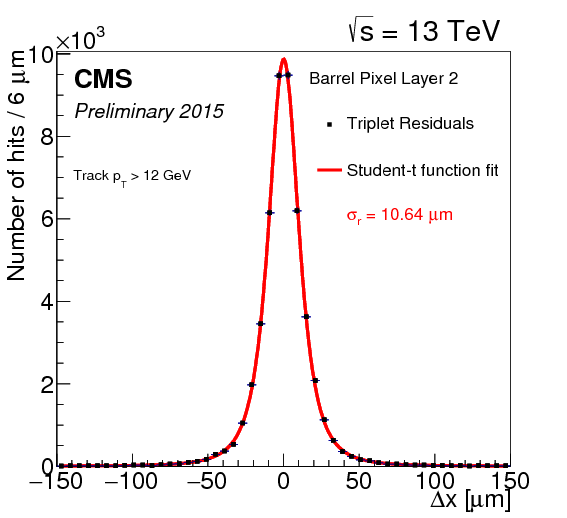
\includegraphics[width=0.5\textwidth]{figures/PixelResolution.png}
  \caption{\label{fig:PixelResolution} Distribution of hit residuals on the second layer of the pixel barrel in the transverse direction to the beam. The distribution is fitted with a student's t-function for which sigma is shown on the plot.}
\end{figure}

\subsection{The Strip Tracker}

The strip tracker is divided into barrel and endcap detectors. The barrel segment is composed of a Tracker Inner Barrel (TIB) section and a Tracker Outer Barrel (TOB) section. The TIB includes four layers of silicon strips each 320 $\mu$m thick and ranging in pitch from 80 $\mu$m and 120 $\mu$m. In the TOB, the lower rate of particle flux allows for larger strips (each 500 $\mu$m thick and ranging in pitch from 120 $\mu$m to 180 $\mu$m).

The endcaps are each comprised of a Tracker Endcap (TEC) and Tracker Inner Disks (TIDs). The TIDs are designed to fill the region between the TEC and the TIB. The TECs each contain nine disks, and each TID contains three disks. On each disk, the modules (for both TID and TEC) are arranged in rings centered on the beam line. Each TID disk contains three rings of modules, while each TEC disk has seven rings. The TID strips (and three innermost ring strips of the TEC) have thickness 320 $\mu$m, while the rest of the TEC strips have thickness 500 $\mu$m. In total the strip tracker contains about 15,400 strip modules. The modules in the innermost two layers of both the TIB and the TOB, as well as the modules in rings 1 and 2 of the TID, and 1, 2 and 5 of the TEC, carry a second strip detector module, which
is mounted back-to-back to the first and rotated in the plane of the module by a ``stereo" angle
of 100 mrad. The hits from these two modules, known as ``$r-\phi$" and ``stereo hits", can be combined
into matched hits that provide a measurement of the second coordinate (z in the barrel and r on
the disks).\cite{TrackReco}\cite{TDR}



\section{The Electromagnetic Calorimeter}

The next layer outward from the silicon tracker is the electromagnetic calorimeter (ECAL), which is designed primarily to measure energies of photons and electrons. The ECAL consists of an array of 75,848 lead tungstate (PbWO$_4$) crystals, and has a barrel (BE) segment as well as two endcap (EE) segments. The BE segment has 61,200 crystals, while each EE segment contains 7,324 crystals. Lead tungstate is highly transparent and is an effective scintillator for photons and electrons, producing light in short, fast, well-defined photon showers that are picked up by photodetectors glued to each crystal. These photodetectors then convert the scintillation light into an electrical signal that can be read out for analysis. 

Each barrel (EB) crystal presents an apparent cross-section (when viewed from the interaction vertex) of $22\times22$  mm$^2$, and are 230 mm (25.8 radiation lengths) thick. The barrel has an inner radius of 129 cm, and covers the pseudorapidity range $0 < |\eta| < 1.479$.\cite{TDR}

The endcap (EE) crystals are each arranged in two D-shaped semicircular aluminum plates. From these plates are cantilevered ``supercrystal" structures consisting of 5x5 crystal blocks. Each crystal presents an apparent cross-section of $28.6\times28.6$ mm$^2$, and are 220 mm (24.7 radiation lengths) thick. The endcap crystals cover the pseudorapidity range $1.479 < |\eta| < 3.0$.\cite{ECAL}

A diagram of the ECAL layout can be seen in Figure~\ref{fig:ECAL_layout}.

\begin{figure}\centering
  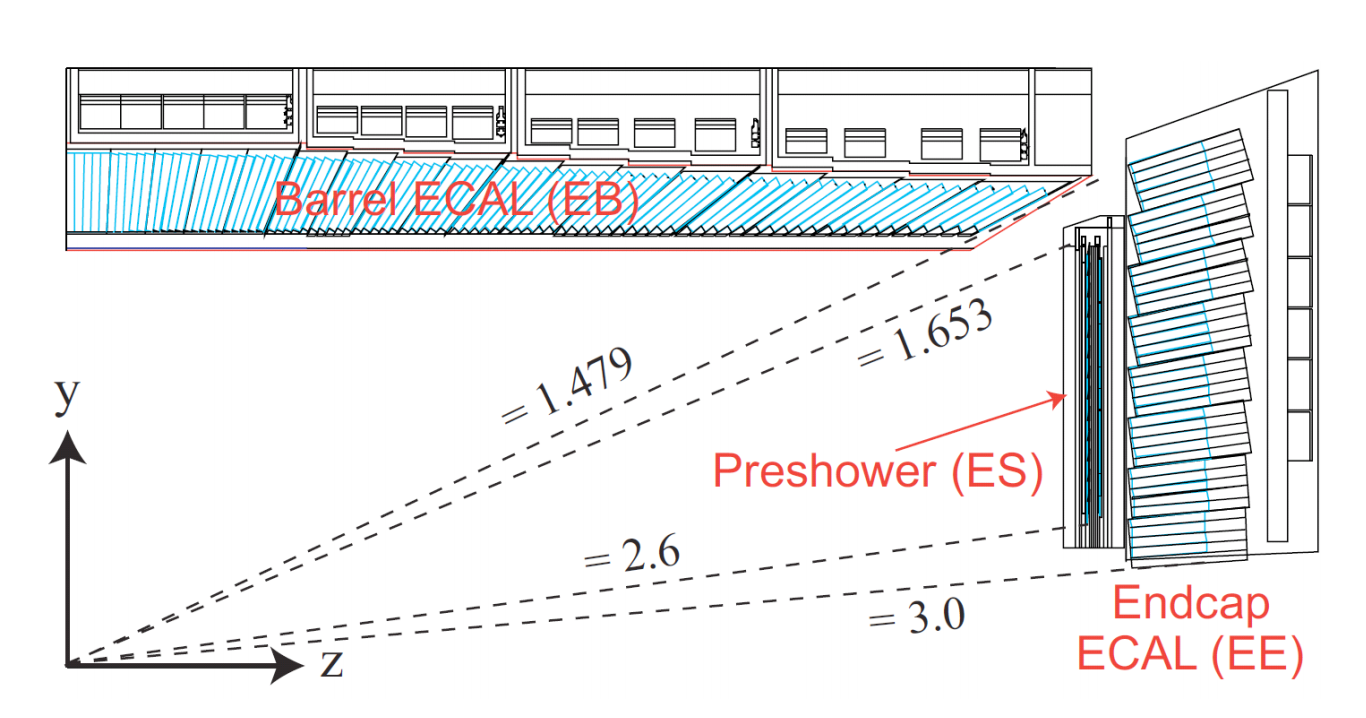
\includegraphics[width=1.0\textwidth]{figures/ECAL_layout.png}
  \caption{\label{fig:ECAL_layout} Layout of the electromagnetic calorimeter (ECAL) indicating the configuration of the barrel (EB) and endcap (EE) crystals. Numbers on the layout are in terms of $\eta$.}
\end{figure}

\subsubsection{ECAL Performance}

In the barrel section of the ECAL, an energy resolution of about 1\% is achieved for unconverted or late-converting photons in the tens of GeV energy range. The remaining barrel photons have a resolution of about 1.3\% up to a pseudorapidity of $|\eta| = 1$, rising to about 2.5\% at $|\eta| = 1.4$. In the endcaps, the resolution of unconverted or late-converting photons is about 2.5\%, while the remaining endcap photons have a resolution between 3 and 4\%~\cite{CMS:EGM-14-001}. When combining information from the entire detector, the jet energy resolution amounts typically to 15\% at 10\GeV, 8\% at 100\GeV, and 4\% at 1\TeV, to be compared to about 40\%, 12\%, and 5\% obtained when the ECAL and HCAL calorimeters alone are used. The energy resolution as a function of pseudorapidity is shown in Figure~\ref{fig:ECAL_Resolution}. \cite{ECAL}

\begin{figure}\centering
  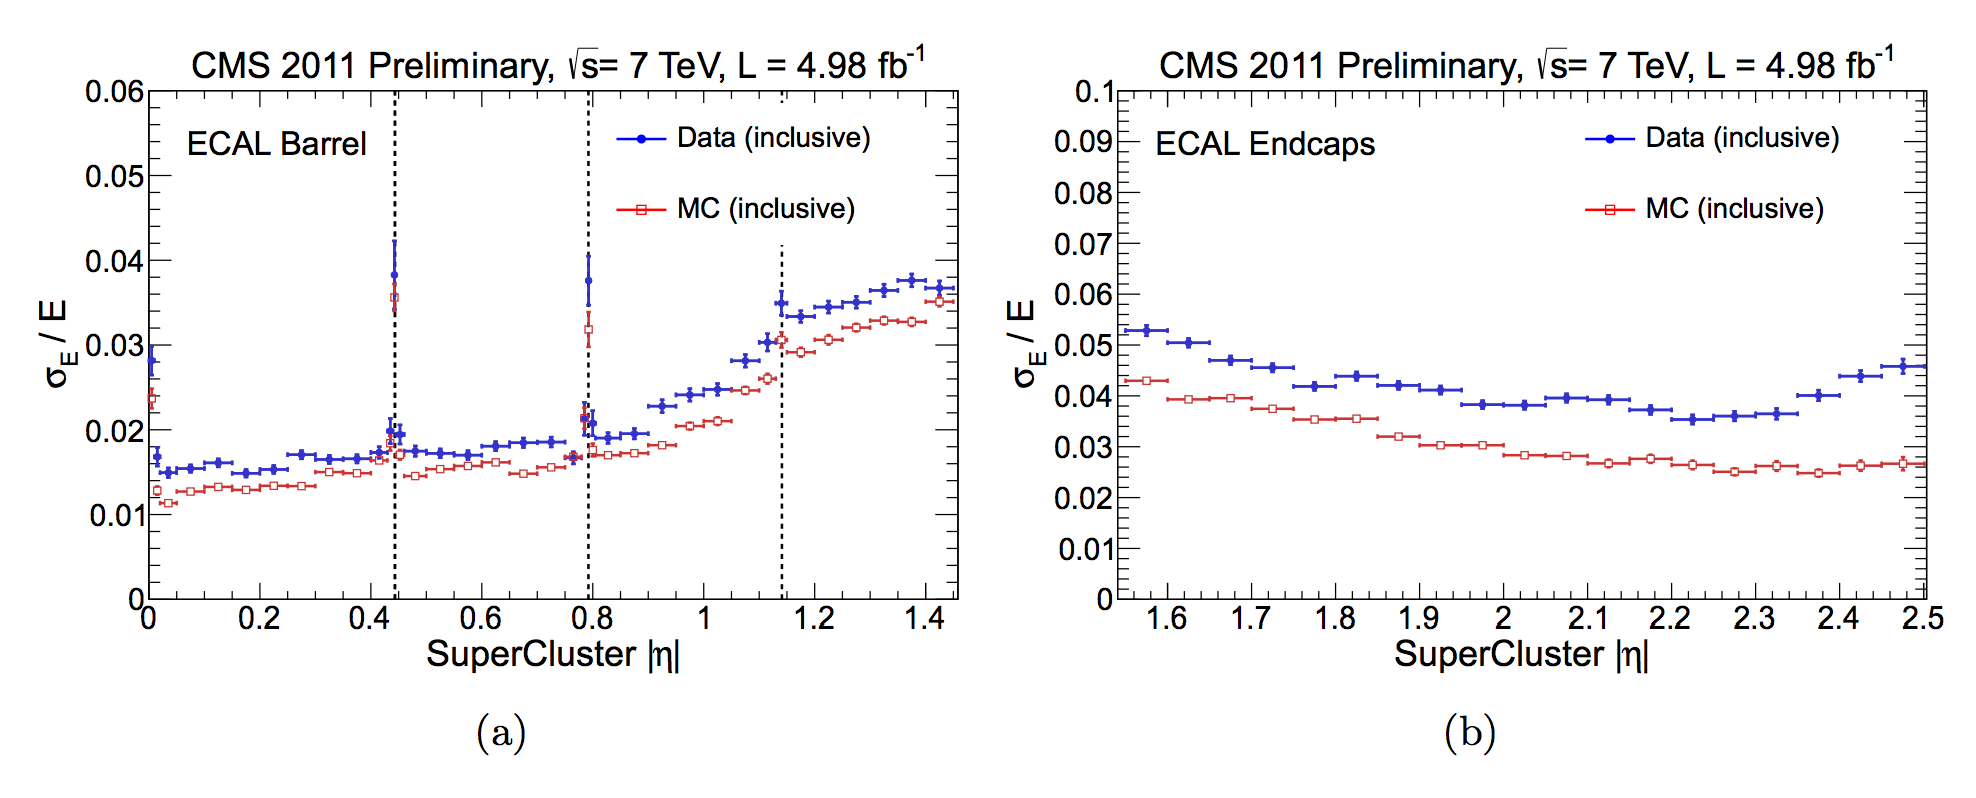
\includegraphics[width=1.0\textwidth]{figures/ECAL_Resolution.png}
  \caption{\label{fig:ECAL_Resolution} Relative energy resolution vs $|\eta|$ in EB (a) and EE (b) for both Monte Carlo and data. The vertical dashed lines indicate module boundaries in EB.}
\end{figure}





\section{The Hadronic Calorimeter}

Surrounding the ECAL is the hadronic calorimeter (HCAL). The primary function of the HCAL is to measure the energies of hadrons (particles composed of quarks). Located just inside the solenoid magnet, the HCAL is primarily composed of brass panels made from melted-down artillery shells. Interspersed with the brass panels are plastic scintillation panels, in which are embedded wavelength-shifting (WLS) fibers, which carry the signal to clear fibers outside the scintillators for readout. As hadrons enter the HCAL, they produce secondary particles in the brass which in turn create further particles. These hadron ``showers" then interact with the plastic scintillators, where the fibers carry the signal to hybrid photodiodes so the signal can be measured.

HCAL is divided into barrel (HB) and endcap (HE) portions. Due to limited space between the ECAL and solenoid, the HCAL also includes material outside the solenoid: the outer HCAL (HO) lining the solenoid, and the forward calorimeter (HF) outside the muon endcap system. The forward hadron (HF) calorimeter uses steel as an absorber and quartz fibers as the sensitive material. The two halves of the HF are located 11.2 m from the interaction region, one on each end, and together they provide coverage in the range 3.0 $< |\eta| <$ 5.2. They also serve as luminosity monitors. These additions increase the total interaction lengths covered by the HCAL to 10.\cite{TDR}

In the region $|\eta| < $ 1.74, the HCAL cells have widths of 0.087 in pseudorapidity and 0.087 in azimuth ($\phi$). In the $\eta$-$\phi$ plane, and for $|\eta| <$ 1.48, the HCAL cells map on to $5 \times 5$ arrays of ECAL crystals to form calorimeter towers projecting radially outwards from close to the nominal interaction point. For $|\eta| >$ 1.74, the coverage of the towers increases progressively to a maximum of 0.174 in $\Delta \eta$ and $\Delta \phi$. Within each tower, the energy deposits in ECAL and HCAL cells are summed to define the calorimeter tower energies, subsequently used to provide the energies and directions of hadronic jets.


A diagram of the HCAL layout is shown in Figure~\ref{fig:HCAL_layout}.

\begin{figure}\centering
  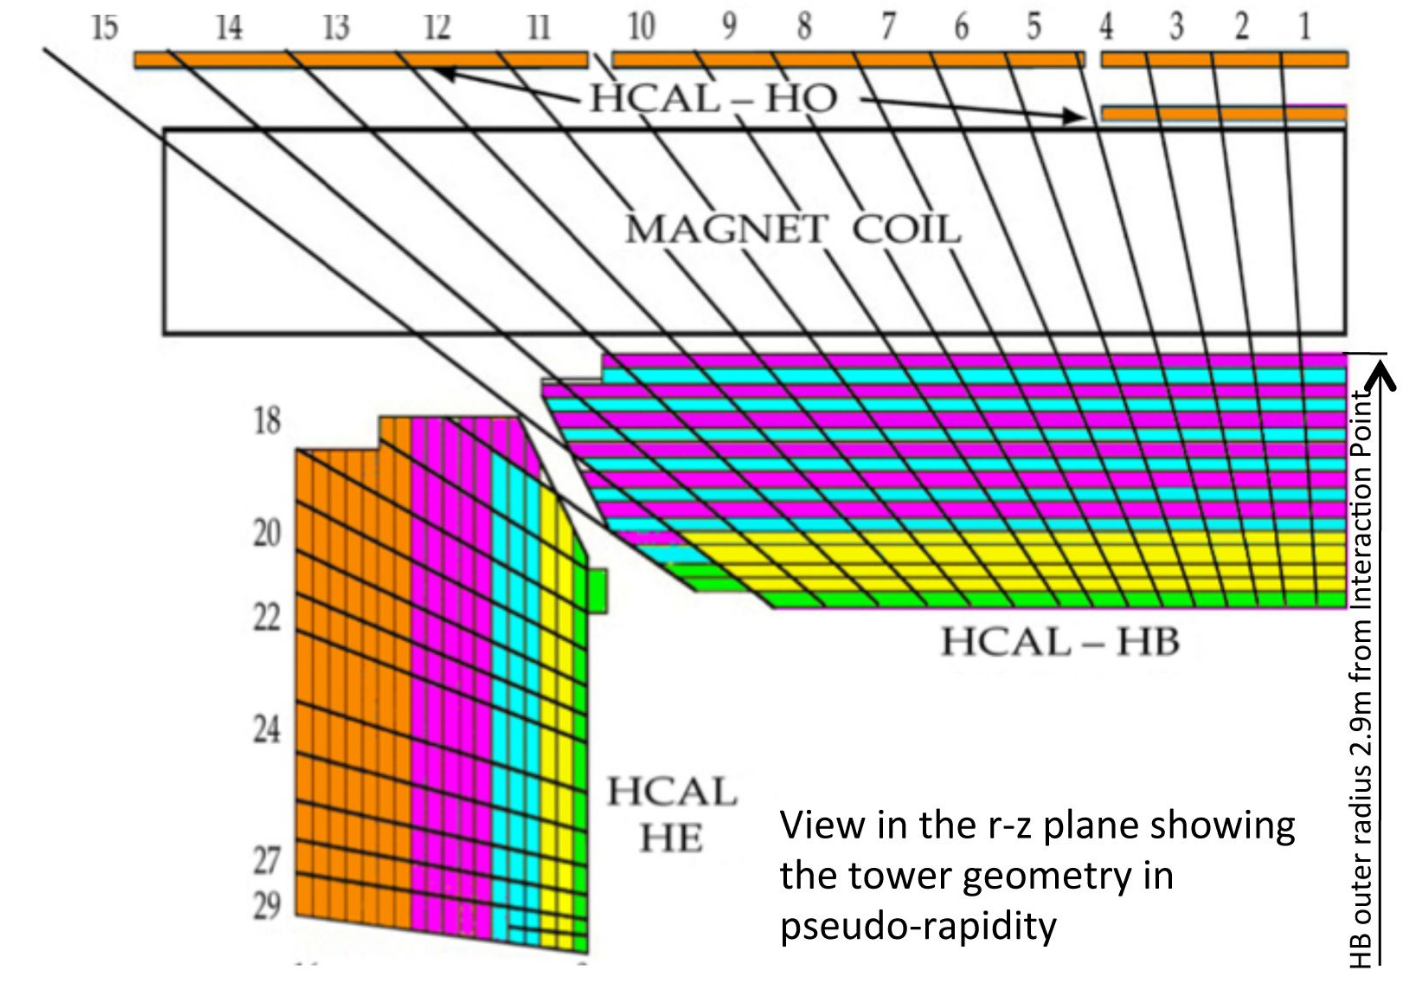
\includegraphics[width=1.0\textwidth]{figures/HCAL_layout.png}
  \caption{\label{fig:HCAL_layout} Layout of the hadronic calorimeter (HCAL) indicating the configuration of the barrel (HB) and endcap (HE) components as well as the outer HCAL (HO) lining the solenoid.}
\end{figure}

\section{The CMS Magnet}

The need to measure high $p_{T}$ muons has driven the requirements on the CMS magnetic field strength. With the goal to determine the momentum of $\approx$1TeV muons with a relative uncertainty of $\approx $10\%, a superconducting solenoid with an interior magnetic field strength of 3.8T was chosen as the central design feature of CMS.

The solenoid is 13 m in length and 6 m in diameter, and is located outside the silicon tracker, ECAL, and HCAL systems, but inside the muon system. Interspersed with the muon system is the steel return yoke, which contains the field outside the solenoid and provides a 2 T field to allow the muon system to measure charged particle momentum. 

To generate the magnetic field, 18,160 amperes are passed through four layers of tightly-wound superconducting Nb-Ti wire, resulting in a stored energy of 2.3 gigajoules.

The magnetic field generated by the solenoid bends charged particles according to the equation
\begin{equation}
R = \frac{p_{T}}{0.3eB}
\end{equation}

\noindent where R is the radius of curvature (in meters), $p_{T}$ is the transverse momentum (in GeV), $e$ is the electron charge (in Coulombs), and $B$ is the field strength (in Tesla). Thus, the transverse momentum ($p_{T}$) of the charged particle can be measured from the known field strength and the observed radius of curvature of the tracks measured in the tracker and muon systems.\cite{TDR}

An artist's rendition of the superconducting solenoid can be seen in Figure~\ref{fig:Solenoid}.

\begin{figure}\centering
  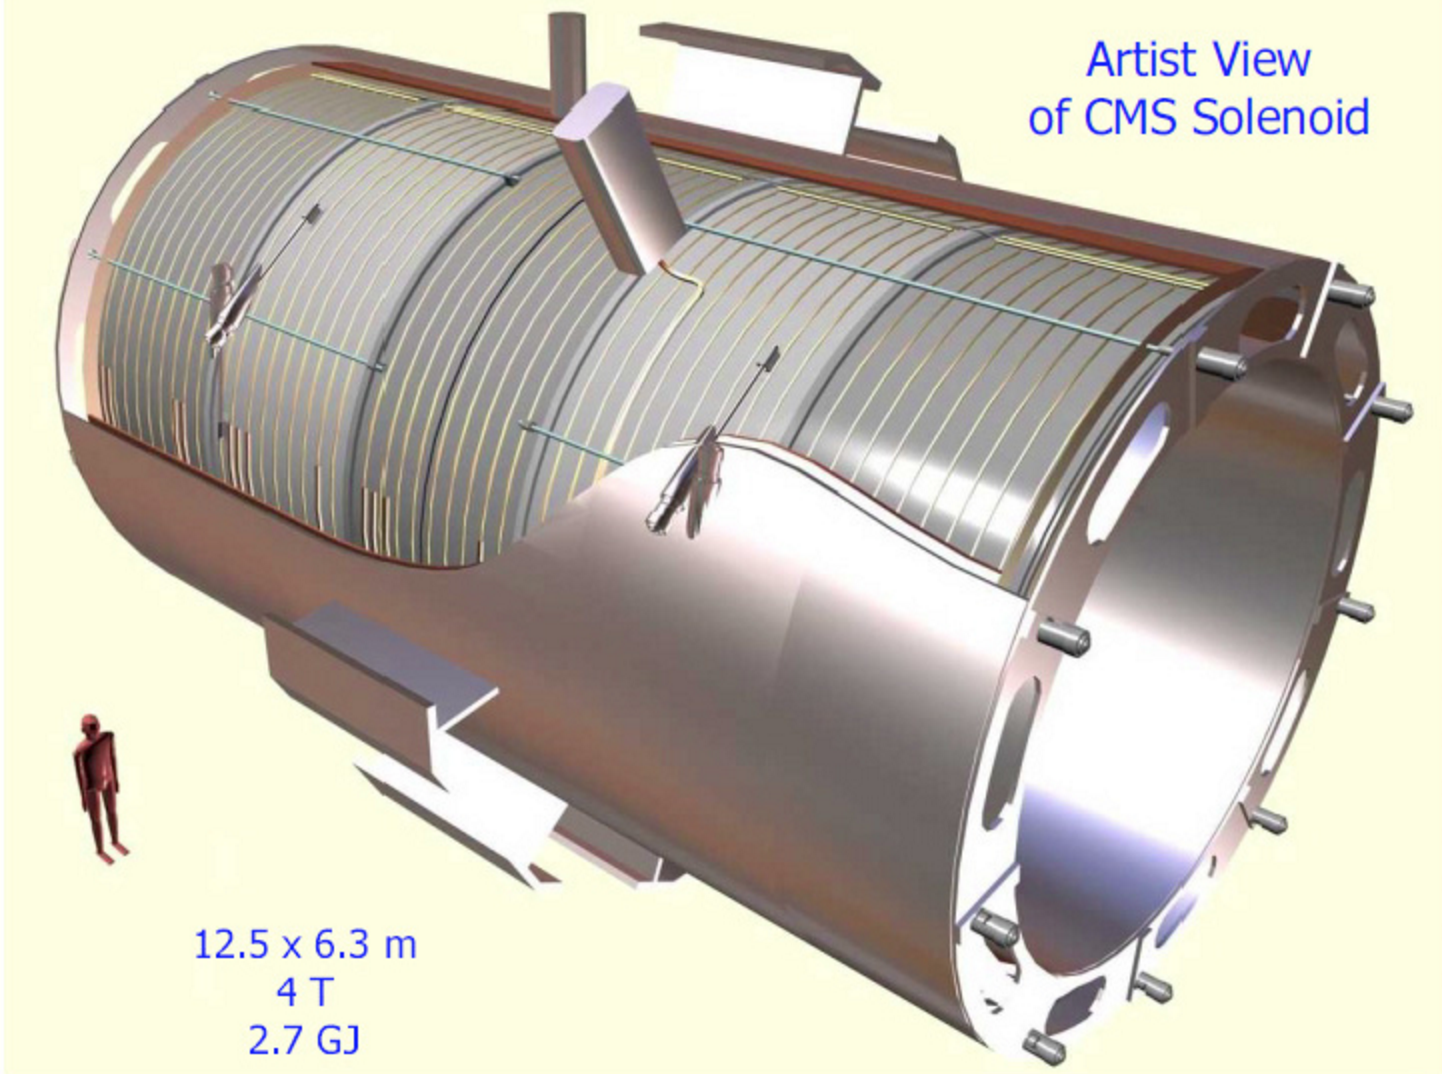
\includegraphics[width=1.0\textwidth]{figures/Solenoid.png}
  \caption{\label{fig:Solenoid} The superconducting solenoid.}
\end{figure}

\section{The Muon System}

The muon system is the outermost subdetector. Muons are measured in the pseudorapidity range $|\eta| <$ 2.4, with detection planes made using three technologies: drift tubes, cathode strip chambers, and resistive plate chambers. Matching muons to tracks measured in the silicon tracker results in a relative transverse momentum resolution for muons with $20 < p_T < 100 \GeV$ of 1.3--2.0\% in the barrel and better than 6\% in the endcaps, The $p_T$ resolution in the barrel is better than 10\% for muons with $p_T$ up to 1\TeV~\cite{Chatrchyan:2012xi}. A diagram of one quadrant of the muon system can be seen in Figure~\ref{fig:muonSystemLayout}. ``MB" indicates the muon barrel subdetector, which is composed of DTs, ``RB" indicates the RPC barrel subdetector, ``ME" indicates the muon endcap subdetector (CSCs), and ``RE" indicates the RPC endcap subdetector. 

An overview of the layout of the muon system can be seen in Figure~\ref{fig:muonSystemLayout}.

\begin{figure}\centering
  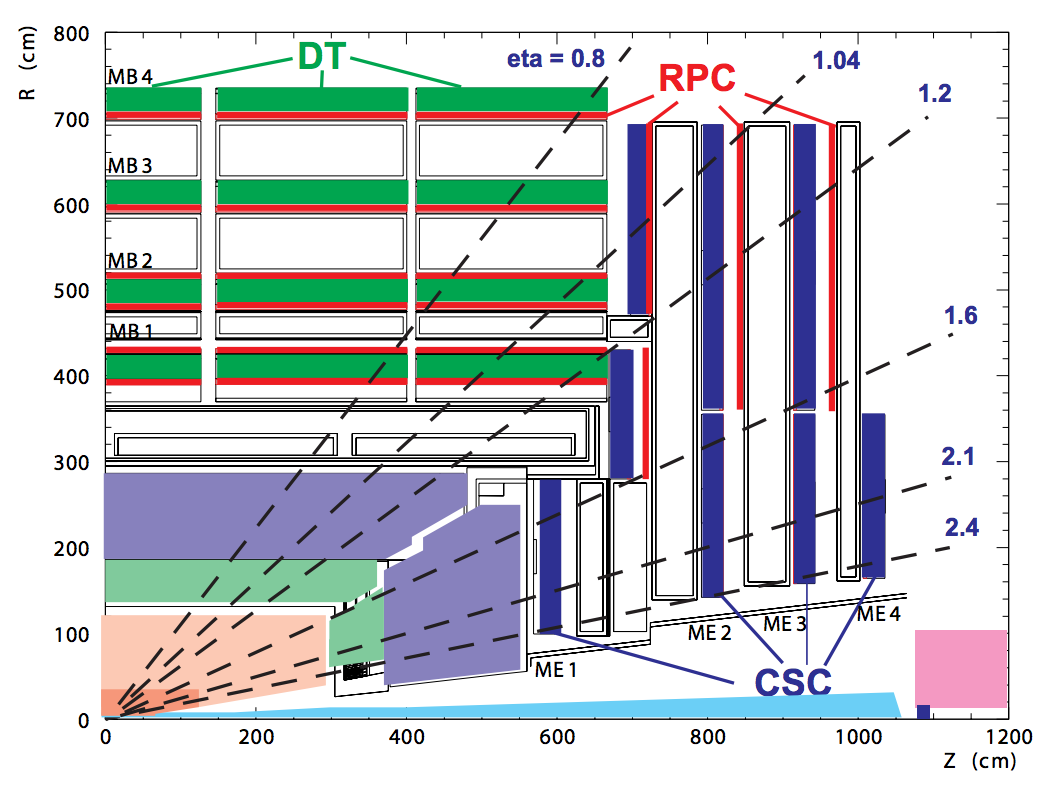
\includegraphics[width=1.0\textwidth]{figures/muonSystemLayout.png}
  \caption{\label{fig:muonSystemLayout} Layout of the muon system highlighting the layered structure of the drift tubes (DTs, green), cathode strip chambers (CSCs, blue), and resistive plate chambers (RPCs, red).}
\end{figure}

\subsection{Drift Tubes (DTs)}

The barrel of the muon system contains 250 layers of DTs arranged in four layers. In the inner three layers, DTs are arranged in 8 $r-\phi$-measuring planes, and 4 $z$-measuring planes. The other layer only contains $r-\phi$-measuring planes.

Each DT is filled with a gaseous mixture of Argon (\~85\%) and carbon dioxide (\~15\%). Charged particles passing through the DT will ionize the gaseous mixture and produce a current along a central filament (upon which a positive voltage is applied) to be read out. The maximum drift length per DT is 2.0 cm and the single point resolution is $\approx$ 200 $\mu$m. By registering where along the wire electrons hit as well as by calculating the muon's original distance away from the wire, DTs give two coordinates for the muon’s position. A plot of DT reconstruction efficiency is given in Figure~\ref{fig:DTEfficiency}.\cite{TDR}

\begin{figure}\centering
  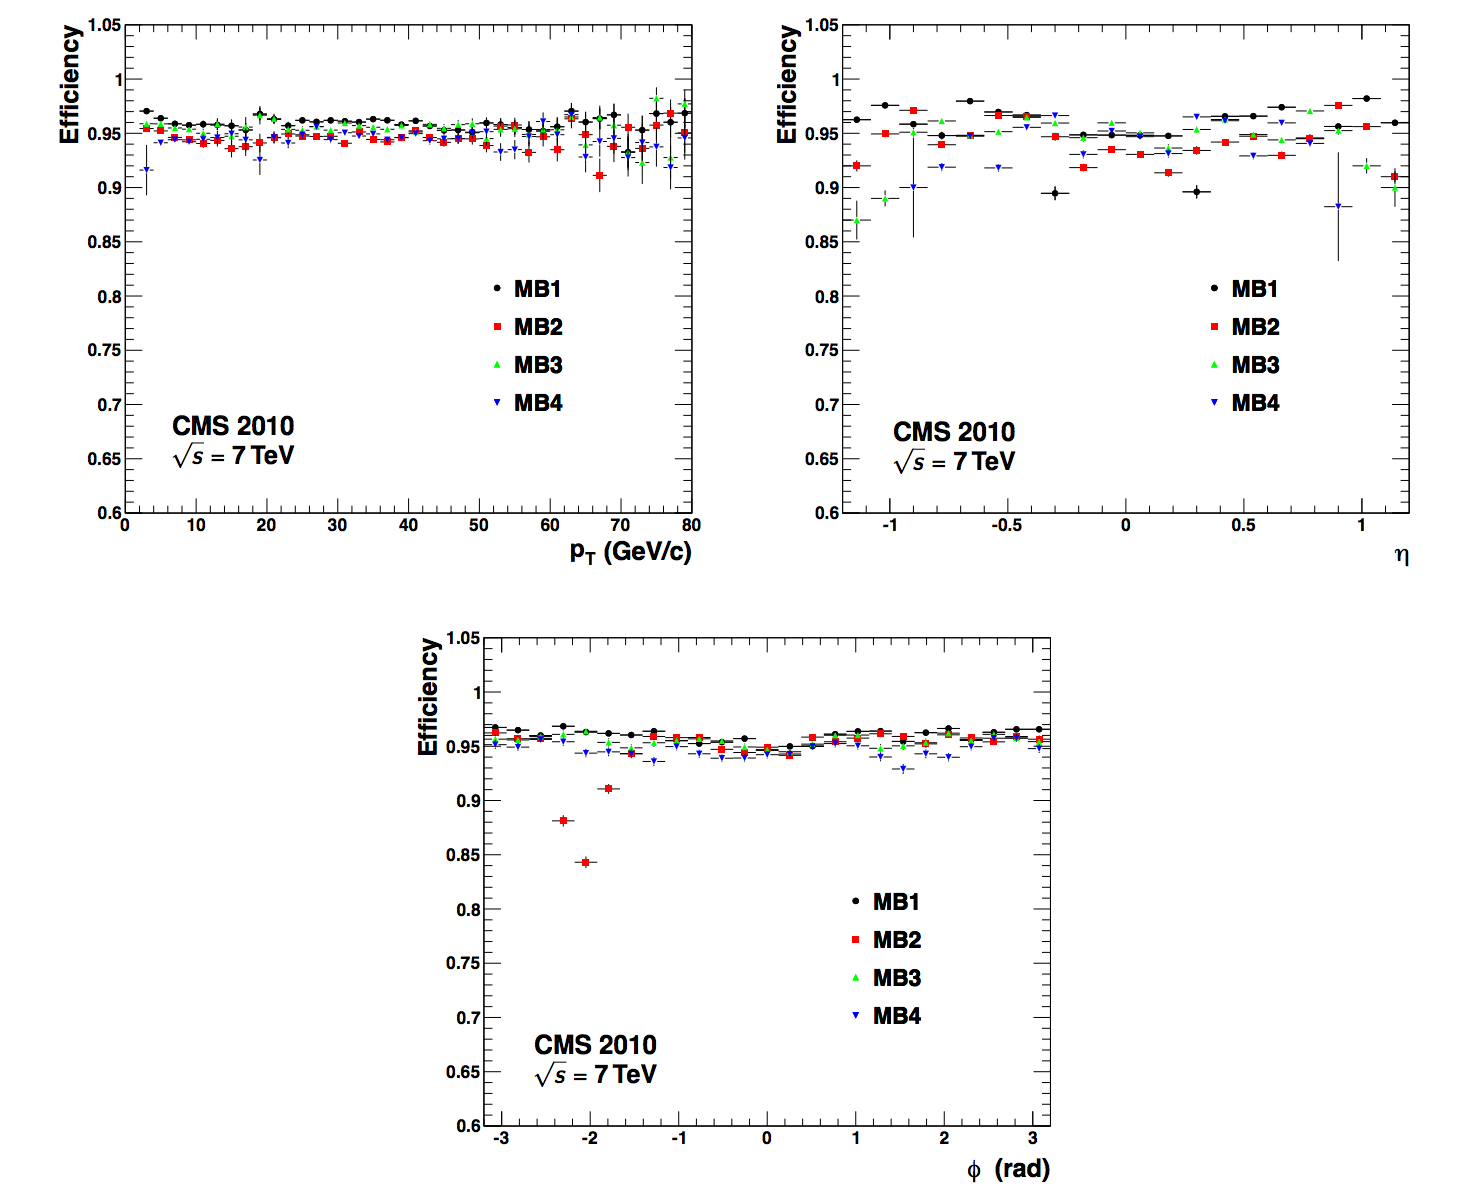
\includegraphics[width=1.0\textwidth]{figures/DTEfficiency.png}
  \caption{\label{fig:DTEfficiency} The measured DT efficiency as a function of the muon transverse momentum $p_T$,
$\eta$, and $\phi$. Results for the 4 stations are superimposed.}
\end{figure}

\subsection{Cathode Strip Chambers (CSCs)}

The muon endcap (ME) system is composed of 234 CSCs in each endcap. The CSCs are trapezoidal in shape and are arranged in four layers. The innermost layer consists of 108 CSCs arranged in three rings of 36 CSCs each. The other layers each have two rings (18 CSCs on the inner ring, 36 on the outer ring, for a total of 54 CSCs per layer).\cite{Muon}

Each CSC is composed of six gas gaps, with each gap containing a radial array of negatively-charged cathode strips and a plane of positively-charged anode wires running perpendicular to the cathodes. The CSCs are overlapped in $\phi$ to avoid gaps in the particle acceptance. When a charged particle ionizes the gas, it leaves a charge on the anode wire and an image charge on a group of cathode strips. The spatial resolution provided from each CSC is $\approx$ 200 $\mu$m. Because the strips and wires are perpendicular, two position coordinates are provided for each passing particle.

The forward (endcap) region of the muon system can expect a higher muon flux, so CSCs were chosen due to their fast response time and fine resolution. Figure~\ref{fig:CSCEfficiency} shows the CSC efficiency, measured using the standard CMS ``tag-and-probe" method, wherein dimuon pairs from $Z$ and $J/\psi$ decays are collected with a single-muon trigger. One muon (the tag) is required to pass standard CMS global muon identification requirements across both the tracker and muon system, while the other muon (the probe) is only required to pass the tracker requirements. The efficiency is measured as the number of ``probe" muons passing the muon system identification requirements divided by the number of ``tag" muons.\cite{Muon}

\begin{figure}\centering
  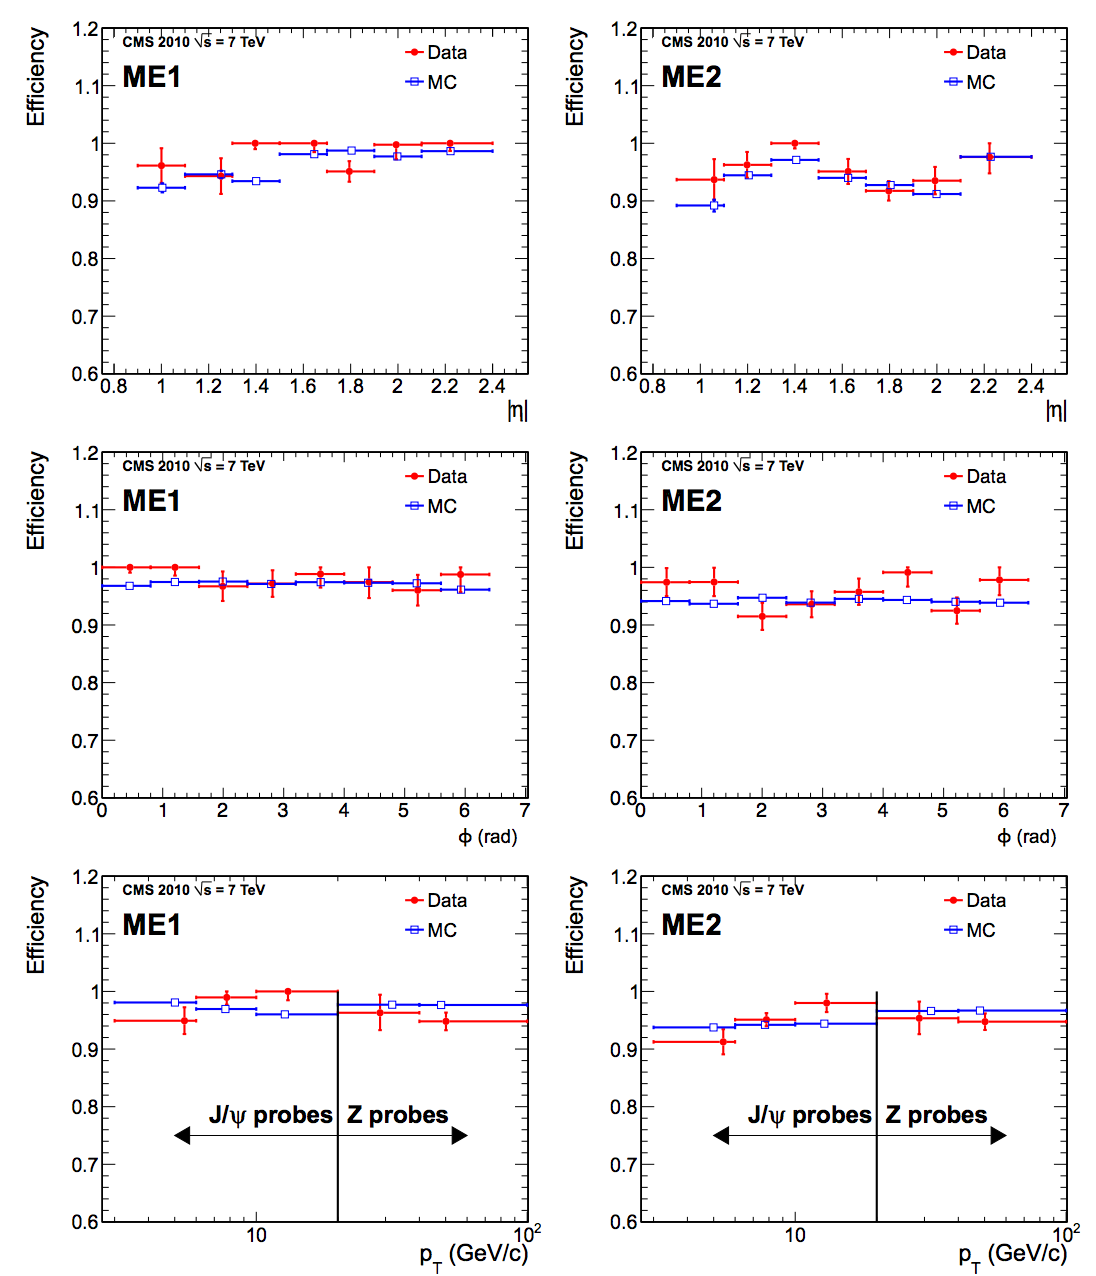
\includegraphics[width=1.0\textwidth]{figures/CSCEfficiency.png}
  \caption{\label{fig:CSCEfficiency} The measured CSC efficiency as a function of $\eta$, $\phi$, and the muon transverse momentum $p_T$ for ME1 (left) and ME2 (right) stations. The vertical lines on the $p_T$ distributions divide the ranges between values covered by the $J/\psi$ and $Z$ probes.}
\end{figure}

\subsection{Resistive Plate Chambers (RPCs)}

RPCs are present in both the barrel and endcaps of the muon system, and are used in parallel with the other two subsystems. The RPCs have timing resolution on the order of nanoseconds and are used primarily to resolve ambiguities in cases of multiple hits in the DTs or CSCs, thereby improving the overall accuracy of particle reconstruction.

There are two layers of RPCs ``sandwiching" each of the first two DT layers (MB1 and MB2), while the outer DT layers (MB3 and MB4) are paired with one RPC each. The endcap CSCs are also paired with one RPC each. 

Each RPC consists of parallel plates of bakelite enclosing two millimeter-thick gas gaps. Each gas gap contains a mixture of 96.2\% R134a (C$_2$H$_2$F$_4$), 3.5\% isobutane (C$_4$H$_10$), and 0.3\% sulfur hexaflouride (SF$_6$). When a muon passes through the chamber, it ionizes the gas and produces a shower of electrons. The bakelite plates are highly transparent to the electrons, which are read out by external metallic strips.

Figure~\ref{fig:RPCResolution} shows an example plot indicating RPC resolution. Similar to pixel resolution, RPC resolution is measured as the residual difference between a ``good" muon track in the muon system and the RPC hits.\cite{Muon}

\begin{figure}\centering
  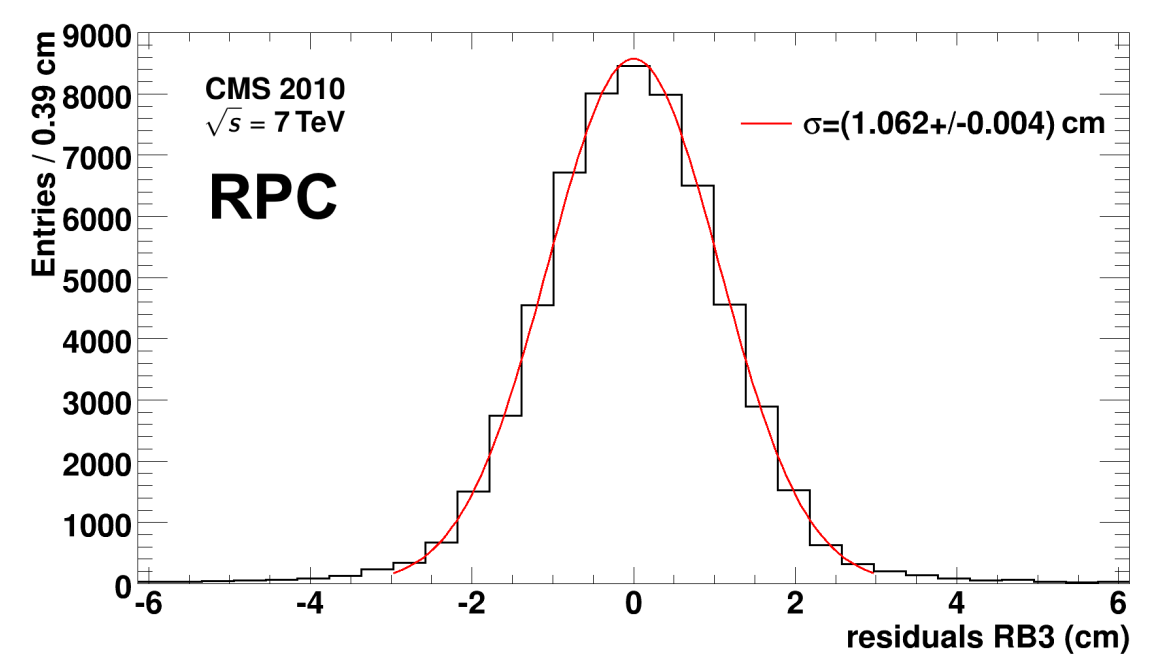
\includegraphics[width=1.0\textwidth]{figures/RPCResolution.png}
  \caption{\label{fig:RPCResolution} Residuals (distance between ``good" track and RPC hit) distribution in RB3 (the RPC associated with MB3 in the barrel of the muon system), fitted to a Gaussian.}
\end{figure}


\section{The Trigger System}

When running at full luminosity, the LHC collides proton bunches at a rate of 40 MHz. With each event requiring $\approx$ 10 MB of digital storage space, this equates to a data-generation rate of 400 TB per second. Since this is obviously unsustainable with current computer storage technology, CMS employs a trigger system to reduce the rate of stored events. Two levels of triggering are used: the hardware-based Level-1 (L1) trigger, which reduces the rate from 40 MHz to approximately 100 kHz, and the hardware-and-software-based High Level Trigger (HLT), which reduces the rate from $\approx$100 kHz to less than 1kHz.\cite{TDR}

\subsection{The Level-1 (L1) Trigger)}

The L1 trigger takes data from the muon system, HCAL, and ECAL in order to make a rapid decision about whether or not to keep the event and send it to the HLT for further review. The L1 trigger latency is about 3.2 $\mu$s, during which time the entirety of the data from the event is temporarily stored. Information from the silicon tracker is not used in this stage of triggering, as the time required by the tracker to reconstruct a track is outside this triggering time window. 

The L1 trigger is divided into three major components: the calorimeter trigger, the muon trigger, and the global trigger. The calorimeter trigger uses the combined (summed) energy deposits in ECAL and HCAL. This information is then passed to the global trigger. The muon trigger uses the DTs, CSCs, and RPCs which in conjunction form the muon system. The muon trigger takes the ``best" four muon candidates from the muon system, where a ``good" muon candidate is defined as having high transverse momentum and a high-resolution track, and passes their information to the global trigger. Using a series of AND-OR algorithms, the global trigger makes the final decision to reject the event or to send it to the HLT.

\subsection{The High level Trigger (HLT)}

The HLT is software-based and uses software-defined ``HLT paths" in order to determine whether or not a given event will pass a particular physics object selection determined by the path. The advantage of this setup is that different HLT paths can be used by different analysis groups studying different physics signatures.

The HLT reconstructs the event from the stored data passed to it by the L1 trigger, and determines whether the event passes a given trigger path. There are four broad categories of HLT path: electrons/photons and muons, jets, missing transverse energy ($\MET$), and taus. Hundreds of specific paths offering high levels of discrimination between required selection criteria are available and grouped into these four categories. As the paths are software-based and not hardware-based, new paths can be customized to the needs of any analysis effort.


\section{Particle Reconstruction}

Even after a given event has passed the L1 trigger and HLT requirements, its constituent particles only exist as hit patterns in the various subdetectors of CMS. In order for any kind of meaningful physics analysis to be performed, these hit patterns must be turned into physics objects which are more easily-read by the CMS software framework (CMSSW). Broadly, the six principal objects that are ``reconstructed" from raw detector data in this manner are: electrons, muons, taus, photons, jets, and missing transverse energy ($\MET$). The chief set of software tools used to reconstruct physics objects is a group of algorithms collectively referred to as Particle Flow (PF).

\subsection{Particle Flow}

The global event reconstruction (also called particle-flow event reconstruction~\cite{CMS-PAS-PFT-09-001,CMS-PAS-PFT-10-001}) consists of reconstructing and identifying each single particle with an optimized combination of all subdetector information. In this process, the identification of the particle type (photon, electron, muon, charged hadron, neutral hadron) plays an important role in the determination of the particle direction and energy. Photons are identified as ECAL energy clusters not linked to the extrapolation of any charged particle trajectory to the ECAL. Electrons are identified as a primary charged particle track and potentially many ECAL energy clusters corresponding to this track extrapolation to the ECAL and to possible bremsstrahlung photons emitted along the way through the tracker material. Muons are identified as a track in the central tracker consistent with either a track or several hits in the muon system, associated with an energy deficit in the calorimeters. Charged hadrons are identified as charged particle tracks neither identified as electrons, nor as muons. Finally, neutral hadrons are identified as HCAL energy clusters not linked to any charged hadron trajectory, or as ECAL and HCAL energy excesses with respect to the expected charged hadron energy deposit.
The energy of photons is directly obtained from the ECAL measurement, corrected for zero-suppression effects. The energy of electrons is determined from a combination of the track momentum at the main interaction vertex, the corresponding ECAL cluster energy, and the energy sum of all bremsstrahlung photons attached to the track. The energy of muons is obtained from the corresponding track momentum. The energy of charged hadrons is determined from a combination of the track momentum and the corresponding ECAL and HCAL energy, corrected for zero-suppression effects and for the response function of the calorimeters to hadronic showers. Finally, the energy of neutral hadrons is obtained from the corresponding corrected ECAL and HCAL energy.
For each event, hadronic jets are clustered from these reconstructed particles with the infrared and collinear safe anti-$k_T$ algorithm, operated with a size parameter $R$ of 0.5, where $R = \sqrt{\eta^2 + \phi^2}$. The jet momentum is determined as the vectorial sum of all particle momenta in this jet, and is found in the simulation to be within 5 to 10\% of the true momentum over the whole \pt spectrum and detector acceptance. Jet energy corrections are derived from the simulation, and are confirmed with in situ measurements with the energy balance of dijet and photon + jet events~\cite{Chatrchyan:2011ds}. The jet energy resolution amounts typically to 15\% at 10\GeV, 8\% at 100\GeV, and 4\% at 1\TeV, to be compared to about 40\%, 12\%, and 5\% obtained when the calorimeters alone are used for jet clustering.

An important quantity related to particle reconstruction is \textit{isolation}. The isolation of a particle is determined by drawing a fixed cone of size parameter $R$ around a particle candidate and summing the energies of all of the other particles as measured in the tracker, ECAL, and HCAL. The most-commonly used definition of isolation is \textit{relative isolation}, $I_{rel}$, which divides the sum of the energy deposits by the \pt of the candidate:
\begin{equation} \label{eq:iso}
I_{rel} = \frac{\sum E_{Tracker} + \sum E_{ECAL} + \sum E_{HCAL}}{p_T(candidate)}
\end{equation}
\noindent Isolation requirements are often standardized by physics object groups (POGs) at CMS. Typically the POG for a given class of particle (e.g. the muon POG), will define a group of isolation ``working points" ranging from loose or very loose to tight. The difference between the working points is typically the maximum value of $I_{rel}$ a candidate must have in order to qualify as a physics object, and the cone size parameter $R$ in which other particles are considered in calculating $I_{rel}$.

The following subsections will detail the methods used to reconstruct each class of particle (except tau leptons, which will be discussed in greater detail in Section \ref{sec:tauID}).

\subsubsection{Track Reconstruction}\label{sec:TrackReco}

The goal of the silicon tracker is to reconstruct tracks showing the trajectories of charged particles through the magnetic field, and furthermore to use these trajectories to ``trace back" the origin of the particle, known as the vertex. The first vertex in each event, that corresponding to the $pp$ collision, is known as the primary vertex (PV). The presence of multiple proton-proton collisions in each bunch crossing, a phenomenon known as pileup, presents the possibility of misidentifying the correct PV for a given event. Therefore, there is a need for a vertexing and tracking algorithms exhibiting a high degree of granularity.

To ensure this, tracks with the highest number of hits in the pixel and strip subsystems within the silicon tracker are recorded (and reconstructed) first. A ``hit" in this case refers to a collection of neighboring strips or pixels registering signal which are grouped into clusters. A particle trajectory can be reconstructed from tracker hits according to the following procedure\cite{TrackReco}:


\noindent\emph{1. Seed generation:} First, all possible combinations of either three hits in the pixel detector or two hits and the beam spot are used to generate a trajectory helix assuming a uniform magnetic field. The \textit{beam spot} is a fixed coordinate representing the average position in x, y, and z of the $pp$ collision over many events. These track seeds are required to pass some minimum $p_T$ threshold and maximum impact parameter threshold, where \textit{impact parameter} or $d_{xy}$ is the minimum distance between the track and either the beam spot or PV.


\noindent\emph{2. Track finding:} Next, the expected trajectories further into the tracker are extrapolated outward from the track seeds. In each subsequent layer, each hit within a $3\sigma$ region around the extrapolated trajectory are fitted using a Kalman filter\cite{Kalman}. The hit with the smallest $\chi^2$ is accepted and the process is repeated in each subsequent layer until the end of the tracker is reached. In cases where a hit is not found in a layer, a ``missing hit" is recorded. Track candidates with more than one missing hit are generally not accepted.


\noindent\emph{3. Track fitting:} In this stage, the requirements on $p_T$ and impact parameter from the seed generation step are removed, and each track candidate is again run through a Kalman filter (refitted). This process starts with the innermost hits and then moves outward through the list of hits, updating the track parameter estimates after each hit.


\noindent\emph{4. Track selection:} This step is designed to reduce the rate of \textit{fake tracks} or reconstructed tracks that are not associated with an actual charged particle. In order to do this, several ``quality cuts" are imposed on the track candidate, such as small impact parameter with respect to a PV (an event may have several PVs due to pileup - in these cases all PVs are considered), low $\chi^2$/dof, and high number of tracker layers with hits.


This tracking procedure is repeated in six total iterations. The first has the most stringent requirements on track $p_T$ and $d_{xy}$, and each following iteration loosens these requirements. After each iteration, the hits corresponding to the tracks reconstructed in the previous iteration are removed for the next iteration.

\subsubsection{Primary Vertex Reconstruction}

Once the tracks in an event are reconstructed, they are then used to estimate each PV in the event. This PV reconstruction is done according to the following procedure\cite{TrackReco}:


\noindent\emph{1. Track selection:} The tracks to be used in the PV reconstruction are selected based on a series of requirements related to track quality as well as likelihood of having been produced in the primary interaction region. These include impact parameter with respect to the beam spot, high number of layers with hits, and low $\chi^2$/dof.


\noindent\emph{2. Track clustering:} A clustering algorithm known as \textit{deterministic annealing} is used to assign the selected tracks to estimated PV candidates. These assignments are made on the basis of both the z coordinate of each track's point of closest approach to the beam spot as well as each track's uncertainty.


\noindent\emph{3. Vertex fitting:} Each track cluster forms a vertex candidate. Those vertex candidates which have at least two associated tracks are used as input to an \textit{adaptive vertex fitter}\cite{AdaptiveVertexFitter}, which outputs the vertex x, y, and z coordinates, position uncertainty, and $\chi^2$.


\subsubsection{Electron Reconstruction}

Electrons are reconstructed via the combination of a track in the silicon tracker and hits in the ECAL towers. These tower hits are called ``superclusters" and their size in $\eta$ and $\phi$ is dictated by various clustering algorithms selected according to the relevant HLT path. As the electron interacts with the silicon in the tracker, it radiates photons via bremsstrahlung. This emission causes the electron to lose momentum and bend further in the magnetic field. To account for this, the supercluster size is tuned to catch these bremsstrahlung photons as well, thereby capturing the total energy of the electron before bending and leading to a more accurate calculation of the electron's energy and momentum. 

To fully reconstruct an electron track, one starts with a track \emph{seed}, which is a possible electron trajectory found by interpolating between layer hits in the pixel and strip detectors. These track seeds must be matched with a supercluster in ECAL. There are two methods to achieve this. The first, ECAL driven seeding, begins by reconstructing superclusters in ECAL and attempts to match them with track seeds in the innermost layer of the pixel detector. The track is then reconstructed from these track seeds. The second, tracker driven seeding, begins with a high-quality track seed and attempts to match it to an appropriate supercluster in ECAL, while also taking into account other clusters arising from bremsstrahlung photons. This is achieved by drawing straight lines tangent to the track towards the ECAL. If a corresponding cluster is found, it is added to the total energy of the electron.

\subsubsection{Muon Reconstruction}

Muons can be measured both in the silicon tracker and the muon system. In order to reconstruct a muon, hits in the muon system (\emph{stand-alone muons}) are matched to hits in the tracker in order to reconstruct a complete muon object, known as a \emph{global muon}. These muons are reconstructed using two different methods, \emph{global muon reconstruction (outside-in)} and \emph{tracker muon reconstruction (inside-out)}.

Global muon reconstruction begins in the muon system. Hits in the DTs and CSCs are allocated into segments, which are short stubs containing just enough hits to assign each a momentum and direction vector. These segments are grouped together to form tracks in the muon system. These tracks, known as stand-alone muon tracks, are matched, one by one, with tracks from the tracker by comparing parameters of the two tracks propagated onto a common surface.

Tracker muon reconstruction begins in the silicon tracker. All tracks with $p_{T} > 0.5$ GeV/c and $p > 2.5$ GeV/c are considered possible muon candidates and are propagated outward toward the muon system, taking into account the magnetic field, expected energy loss, and the possibility for multiple Coulomb scattering in the detector material. If a hit in the muon system is found within 3 cm in local $x, y$ coordinates, the candidate qualifies as a tracker muon.

Tracker muon reconstruction is more efficient than global muon reconstruction at low energies ($p < 5$ GeV/c), since it only requires a single muon hit in the muon system. Global muon reconstruction is more appropriate for muons with higher energies penetrating through more than one station in the muon system.


\subsubsection{Photon and Neutral Hadron Reconstruction}

Since photons and neutral hadrons are chargeless, and therefore leave no hits in the silicon tracker, their reconstruction takes place in ECAL (photons) and HCAL (hadrons). The identification of photons and neutral hadrons takes place via \textit{clustering algorithms} which are designed to separate photons from neutral as well as charged hadrons, and to differentiate photons originating from the primary or secondary vertices from those generated by electrons undergoing bremsstrahlung. Photons may also convert into e$^+$e$^-$ pairs in the tracker, and further clustering algorithms have been developed in order to capture these conversions and factor them into the photon reconstruction.

Clustering algorithms in ECAL involve three steps. First, a seed cluster is identified in one of the ECAL towers as a tower with a local energy maximum passing a threshold specified by the algorithm. Next, topological clusters are defined as clusters adjacent to (sharing at least one side in common with) the seed cluster and with cell energies passing another threshold. These thresholds are generally set to be two standard deviations above the base electronics noise level in each of the separate ECAL segments (80 MeV in the barrel and 300 MeV in the endcaps). Finally, topological clusters then generate as many ``particle flow" clusters as there are seed clusters, and the energy in each particle flow cluster is allocated according to its distance from the seed. Furthermore, in particle flow, ECAL clusters are required \emph{not} to match any tracks in the tracker in order to qualify as photon candidates. Similarly, neutral hadrons are identified by the presence of clusters in HCAL with no corresponding track.


\subsubsection{Jet Reconstruction}

Jets are primarily reconstructed in ECAL and HCAL, although their charged constituents usually leave tracks in the silicon tracker as well. The majority of reconstructed jet energy comes from charged particles such as pions and kaons, and a smaller but still sizable portion comes from photons from $\pi^0$ decays in ECAL. Jets are reconstructed offline from the energy deposits in the calorimeter towers, clustered by the anti-$k_\mathrm{t}$ algorithm~\cite{Cacciari:2008gp, Cacciari:2011ma} with a size parameter of 0.5. In this process, the contribution from each calorimeter tower is assigned a momentum, the absolute value and the direction of which are given by the energy measured in the tower, and the coordinates of the tower. The raw jet energy is obtained from the sum of the tower energies, and the raw jet momentum by the vectorial sum of the tower momenta, which results in a nonzero jet mass. The raw jet energies are then corrected to establish a relative uniform response of the calorimeter in $\eta$ and a calibrated absolute response in transverse momentum \pt.

\subsubsection{Missing Transverse Energy}

The colliding protons in the LHC have zero net transverse momentum. By conservation of momentum, it's expected that the particles generated from each $pp$ collision will have net zero total transverse momentum. Some of these particles will evade CMS undetected, however. The sum of their momenta is known as missing transverse energy, denoted as $\MET$. Since we must have $\sum_{detected particles} \vec{p_T} + \sum_{undetected particles} \vec{p_T} = 0$, we can express the $\MET$ as
\begin{equation} \label{eq:METCalc}
\MET = - \sum_{detected particles} \vec{p_T}
\end{equation}

CMS employs multiple definitions of $\MET$, but the one used in this thesis is \textit{particle flow $\MET$}, or \textit{PF-$\MET$}. PF-$\MET$ uses all particle-flow objects as well as all available detector information in calculating the $\MET$ according to Equation \ref{eq:METCalc}.
